\documentclass{article}
\usepackage{a4wide}
\usepackage{graphicx}
\pagestyle{headings}

\begin{document}
\title{\textbf{Software Project Management Plan}\\ for \textit{Earth} Project}\author{Alex Egan \\ Callum Baillie \\ George Sainsbury \\ Hill-Jian Huang \and Ming Jie Tan \\ Jonathan Velasco \\ Sahil Choujar \\ Yang Qing \\ Ken S'ng Wong \and Filimoni Lutunaika \\ Mohammad Bamogaddam \\ Kun Zhou \\ Xiaodong Cui \\ Hemant Singh }

\maketitle
\thispagestyle{empty}
\newpage{}

\thispagestyle{empty}
\tableofcontents
\newpage{}

\setcounter{page}{1}

\section{Introduction}

\label{sec:intro}

\subsection{Purpose and Scope}

This project endeavours to build upon the existing framework that has already been developed for \textit{Earth}. Currently there exist a number of features that would be desirable to be implemented in this open source software. It is our aim to implement as many features as is necessary to further evolve Earth into a highly manageable and efficient tool.\\
\\
This document outlines the direction the project will take to best deliver the final product. In other words, this document will show how our team is assigned to deal with the task required of us. This project management plan looks at how we will deal with risks and how they will be mitigated and how they will be controlled should they arise. Furthermore, we show how we intend to develop additional features of Earth, showing not only the process model that we will use but also how the work is scheduled to take place.

\subsection{Project Deliverables}

The following section outlines when specific documents and deliverables will be completed and available. These are the main deliverables. However, more detailed information about internal milestones are provided in Section \ref{sec:work-plan}.

\subsubsection{First Document Drafts}

\begin{enumerate}
\item Software Project Management Plan - due 31/03/08
\end{enumerate}

\subsection{Evolution of the Plan}

This plan will be reviewed on a weekly basis for the duration of the project. In addition to these regular updates, every time our work on the project differs to the proposed workplan, this document will be updated as necessary. These changes may be made by any member of the group. To ensure that the project stays on track, along with this document, there are numerous risk management procedures in place. Furthermore, with regular meetings, we are able to stay aware of where we are compared to where we should be as set out by our milestones and deliverables.\\

\section{References}

\textit{Software Engineering} 8th Ed., I. Sommerville, Addison-Wesley, 2007\\

\section{Definitions}

Following is a table of acronyms and their meanings.

\begin{table}[htp]
\begin{centering}
\begin{tabular}{| l | l |}
\hline 
CASE & Computer Assisted Software Engineering\\
SVN & Subversion\\
SPMP & Software Project Management Plan\\
\hline
\end{tabular}
\par\end{centering}


\caption{Acronyms}
\end{table}


\section{Project Organisation}

\subsection{Roles and Responsibilities}
\label{roles-and-responsibilities}
This project group has been divided up such that we have three development teams. Each team will be assigned their own tasks to complete, and testing of each individual component will be completed by the group that it was assigned to. This group structure allows for the members of each individual group to focus on development of their tasks and not have to worry about dealing with organisation.

\subsubsection*{Minutes: Ken S'ng Wong}
George has taken on the task of taking and managing the minutes for all formal meetings.

\subsubsection*{Git Management Team: Alex Egan, Ken S'ng Wong, Mohammad Bamogaddam}
This group manages the git repository structure for the entire group as well as maintaining each development team's repository and the document repository.

\subsubsection*{Primary Meeting Chairperson: Ming Tan}
Ming is organising agendas and chairing the meetings. However at times other members may take on his role, in the event this does happen, it will be noted in the agenda.

\subsubsection*{Development Team 1 - Gui and Testing Development}
Development Team 1 consists of George Sainsbury, Alex Egan, Xiaodong Cui and Filimoni Lutunaika.

\subsubsection*{Development Team 2 - Plugin Development}
Development Team 2 consists of Ming Tan, Callum Ballie, Kun Zhou, Mohammad Bamogaddam and Yang Qing. Development Group 2 will also facilitate the documentation of this project.

\subsubsection*{Development Team 3 - Database Development}
Development Team 3 consists of Jonathan Velasco, Sahil Choujar, Ken S'ng Wong, Hemant Singh and Hill-Jian Huang.
\\

\newpage

\section{Risk Management Plan}

Detailed below are various risks that may affect the project and strategies for dealing with them.

\subsection{Staff unable to work due to sickness}
\begin{itemize}
	\item \textbf{Likelihood:} Moderate as Staff are vulnerable to various diseases such as the flu.
	\item \textbf{Severity:} It could be catastrophic if the absence is for a long period of time as some staff possess specialised knowledge in specific areas. However, if the time of absence is short, the severity will be tolerable.
	\item \textbf{Indicators:}
		\begin{itemize}
			\item Advanced notice from the staff member who will be unavailable or unable to work 
			\item Staff member does not attend meetings.
			\item Staff member complains about their health
		\end{itemize}
	\item \textbf{Strategies:} 
		\begin{itemize}
			\item Organise staff to work in teams so that more than one person understands and can work on each task. This allows the team to continue working even if a member is unable to work.
			\item Provide time slack on all tasks so that other members have enough time to pick up the jobs of those unable to work.
		\end{itemize}
\end{itemize}

\subsection{Staff unable to work due to other commitments}
\begin{itemize}
	\item \textbf{Likelihood:} Moderate as staff may have unexpected commitments such as business or family trips.
	\item \textbf{Severity:} It could be catastrophic if the absence is for a long period of time as some staff possess specialised knowledge in specific areas. However, if the time of absence is short, the severity will be tolerable.
	\item \textbf{Indicators:}
		\begin{itemize}
			\item Advanced notice from the staff member who will be unavailable or unable to work  
			\item Staff member does not attend meetings.
		\end{itemize}
	\item \textbf{Strategies:} 
		\begin{itemize}
			\item Organise staff to work in teams so that more than one person understands and can work on each task. This allows the team to continue working even if a member is unable to work.
			\item Provide time slack on all tasks so that other members have enough time to pick up the jobs of those unable to work.
		\end{itemize}
\end{itemize}

\subsection{Difficulty in adding features due to poor software design in existing code}
\begin{itemize}
	\item \textbf{Likelihood:} Moderate as the code was likely developed to meet existing needs without foresight for unexpected but desired improvements.
	\item \textbf{Severity:} High as the time necessary to fix any design issues in the existing code to implement certain features could increase significantly.
	\item \textbf{Indicators:}
		\begin{itemize}
			\item Problems when attempting to design a feature to be implemented around the existing code.
		\end{itemize}
	\item \textbf{Strategies:} 
		\begin{itemize}
			\item Attempt to avoid features that may not be easily integrated with the existing code.
			\item Redesign of certain sections of existing code to implement new feature.
		\end{itemize}
\end{itemize}

\subsection{Unable to contact Rising Sun Pictures to Clarify Requirements}
\begin{itemize}
	\item \textbf{Likelihood:} Medium as the main developers of earth are situated at the Sydney office.
	\item \textbf{Severity:} Medium because it will not allow for certain requirements that require clarification to proceed until contact is made.
	\item \textbf{Indicators:} 
		\begin{itemize}
			\item Lack of email response.
			\item Advanced notice that their offices are busy.
		\end{itemize}
	\item \textbf{Strategies:} 
		\begin{itemize}
			\item Proceed to other already clarified requirements.
			\item Prepare numerous requirements to clarify during meetings with Rising Sun Pictures.
		\end{itemize}
\end{itemize}

\subsection{Lack of knowledge of Ruby, Rails, Git}
\begin{itemize}
	\item \textbf{Likelihood:} The likelihood is high as all of the above tools are new to the development team.
	\item \textbf{Severity:} The severity is catastrophic as it would be extremely difficult to finish the project on time and with a high level of quality without knowledge of the tools.
	\item \textbf{Indicators:}
		\begin{itemize}
			\item Slow adoption of required set of tools upon selection
			\item Staff member complains about any of these tools
			\item Selection of these tools late, having reduced time to study them
		\end{itemize}
	\item \textbf{Strategies:} 
		\begin{itemize}
			\item Inform the development team that these are the tools to be used in advance so that they have time learn to use them.
			\item Organise a tutorial or lectures of these tools and its functionality to show the developers how to use the tools and what they can be used for.
			\item Include time in the schedule for learning how to use these tools and their functionality.
		\end{itemize}
\end{itemize}

\subsection{Requirements not completed on time - excessive number of requirements}
\begin{itemize}
	\item \textbf{Likelihood:} The likehood is moderate as the requirements selection is done internally.
	\item \textbf{Severity:} High as features intended for the final product will not be completed.
	\item \textbf{Indicators:}
		\begin{itemize}
			\item The number of requirements is too large.
			\item Clients continue adding more requirements
			\item Lack of sufficient communication between the development team and the clients causing the wrong requirements to be implemented.
		\end{itemize}
	\item \textbf{Strategies:} 
		\begin{itemize}
			\item Have the development team and the clients meet regularly to review the requirements and the progress of their implementation.
			\item Maximize the detail of the requirements in the SRS.
			\item Develop the project in such a way that adapting to new or changed requirements is easy. 
		\end{itemize}
\end{itemize}

\subsection{Requirements not completed on time - unreachable complexity of the requirements}
\begin{itemize}
	\item \textbf{Likelihood:} The likehood is high as it is likely that after delving into the existing code, that implementing a feature could become a much larger problem. 
	\item \textbf{Severity:} High as the system may be unable to work correctly or may behave in an incorrect or inefficient manner.
	\item \textbf{Indicators:} 
		\begin{itemize}
			\item The level of difficulty of the implementation of the requirements is too high.
			\item Lack of sufficient communication between the development team and the clients causing the wrong requirements to be implemented.
		\end{itemize}
	\item \textbf{Strategies:} 
		\begin{itemize}
			\item Have the development team and the clients meet regularly to review the requirements and the progress of their implementation.
			\item Maximize the detail of the requirements in the SRS.
			\item Develop the project in such a way that adapting to new or changed requirements is easy. 
		\end{itemize}
\end{itemize}

\subsection{Underestimate the development time to reach each milestone}
\begin{itemize}
	\item \textbf{Likelihood:} The likelihood is medium as initial estimates of task time may be incorrect, and result in needing more time. 
	\item \textbf{Severity:} High as the project may be not delivered on time or may not reach the required quality level. 
	\item \textbf{Indicators:}
		\begin{itemize}
			\item Milestones not met on time.
			\item Requirements changing constantly.
		\end{itemize}
	\item \textbf{Strategies:} 
		\begin{itemize}
			\item Increase the free slack time of each milestone in order to have some extra time if needed.
			\item Reassign members/development teams to increase the speed at which the core components are completed.
		\end{itemize}
\end{itemize}

\subsection{New features of the project do not integrate correctly with Earth}
\begin{itemize}
	\item \textbf{Likelihood:} The likelihood will depend on the level of integration required and how interconnected a component is. Therefore, the likelihood can vary from low to high.
	\item \textbf{Severity:} Moderate as time to analyse and fix problems may delay the feature being implemented
	\item \textbf{Indicators:} Feature doesn't work as intended with Earth
	\item \textbf{Strategies:} 
		\begin{itemize}
			\item Have input from multiple developers when designing components
			\item Begin integration early so that there is more time to deal with any problems that occur
			\item Have incremental integration with smaller components so that problems are easier to identify
		\end{itemize}
\end{itemize}

\subsection{Unable to work at the computer labs}
\begin{itemize}
	\item \textbf{Likelihood:} Medium because while there are many labs, not all systems will have the necessary tools for this project.
	\item \textbf{Severity:} Low because it is not required to work in the computer labs.
	\item \textbf{Indicators:} 
		\begin{itemize}
			\item Advance notice that the computer labs will not be available.
			\item No computers are available due to maintenance or use by other people
		\end{itemize}
	\item \textbf{Strategies:} 
		\begin{itemize}
			\item Install the required tools on other computers or use remote access to computers that have the required tools.
			\item Install the required tools on computers in the SEP Labs.
		\end{itemize}
\end{itemize}

\subsection{Central Earth Git repository unavailable}
\begin{itemize}
	\item \textbf{Likelihood:} Low as maintenance of the Git repository and its availability is the responsibility of a separate department.
	\item \textbf{Severity:} Low as each developer has their own copy of the Git repository to work on.
	\item \textbf{Indicators:} 
		\begin{itemize}
			\item Degraded performance.
			\item Scheduled downtime or maintenance.
		\end{itemize}
	\item \textbf{Strategies:} 
		\begin{itemize}
			\item Continued Development on local copies of the repository, with progress to be pulled/pushed once the repository is restored.
			\item Keep the number of files to a minimum by splitting work into groups and sections.
		\end{itemize}
\end{itemize}

\newpage

\section{Process Model}

Agile Process will be adopted for this project. This entails short development cycles, with many milestones to be met. In general we will adopt a 6 week development sprint, where requirements investigation and prototyping will occupy 1 week, with 3 weeks of development time and 1-2 weeks of testing time. This allows for developed and tested products and endorses incremental development.
\\

\section{Work Plan}
\label{sec:work-plan}

This project makes use of an iterative process where the existing code will be improved upon with additional features.
\\
The time estimates provided show the average duration of time that each member assigned to the task spends on that task.

\subsection{Milestone 1 - Work Activities}

\begin{itemize}
\item Infrastructure
\item Documentation
\item Ticket 27
\item Ticket 66
\item Ticket 75
\item Ticket 120
\item Ticket 127
\item Ticket 145
\item Testing
\end{itemize}

\subsubsection{Infrastructure}
	This task involves the installation of Earth along with ruby and rails, and ensuring that any code changes can be integrated, compiled and tested. As such it is to be undertaken by all group members.\\
	
	Resource: All Development Staff
	Time Estimate: 5hrs

\subsubsection{Documentation}
	This involves the development and maintenance of existing documents for the project plan and any subsequent documents.\\
	
	Resource: Ming Tan
	Time Estimate: 8hrs

\subsubsection{Ticket 27}
	This ticket involves figuring out and recording of the filetypes of files in the database.\\
	
	Resource: Development Group 3 (Jonathan Velasco, Sahil Choujar, Ken S'ng Wong, Hemant Singh and Hill-Jian Huang)
	Time Estimate: 4hrs

\subsubsection{Ticket 66}
	This ticket involves the listing of space used by each user.\\
	
	Resource: Development Group 3 (Jonathan Velasco, Sahil Choujar, Ken S'ng Wong, Hemant Singh and Hill-Jian Huang)
	Time Estimate: 4hrs

\subsubsection{Ticket 75}
	This ticket involves the sorting of directory and file listings by name and size.\\
	
	Resource: Development Group 1 (George Sainsbury, Alex Egan, Xiaodong Cui, Filimoni Lutunaika )
	Time Estimate: 4hrs

\subsubsection{Ticket 120}
	This ticket involves the display of green bars for sizes in the "All Files" view.\\

	Resource: Development Group 2 (Ming Tan, Callum Ballie, Kun Zhou, Mohammad Bamogaddam and Yang Qing)
	Time Estimate: 4hrs
	
\subsubsection{Ticket 127}
	This ticket involves the display of a warning should the user's browser not be SVG capable when attempting to view SVG.\\
	
	Resource: Development Group 2 (Ming Tan, Callum Ballie, Kun Zhou, Mohammad Bamogaddam and Yang Qing)
	Time Estimate: 4hrs

\subsubsection{Ticket 145}
	This ticket requires the relabelling of file sizes from  "> 0 TB" to something more meaningful.\\
	
	Resource: Development Group 1 (George Sainsbury, Alex Egan, Xiaodong Cui, Filimoni Lutunaika )
	Time Estimate: 4hrs
	
\subsubsection{Testing}
	Testing will be conducted on each of the tickets above, and testing scripts or unit tests will be created as necessary.\\
	
	Resource: All Development Groups
	Time Estimate: 8hrs

\subsubsection{Milestone 1 - Schedule Allocation}

The milestones and tasks are shown graphically in Figure \ref{fig:schedule} below. This figure shows the relative times between the deadlines of the tasks required and also shows the estimated time for the completion of each individual tasks.\\

\begin{figure}[htp]
\begin{centering}
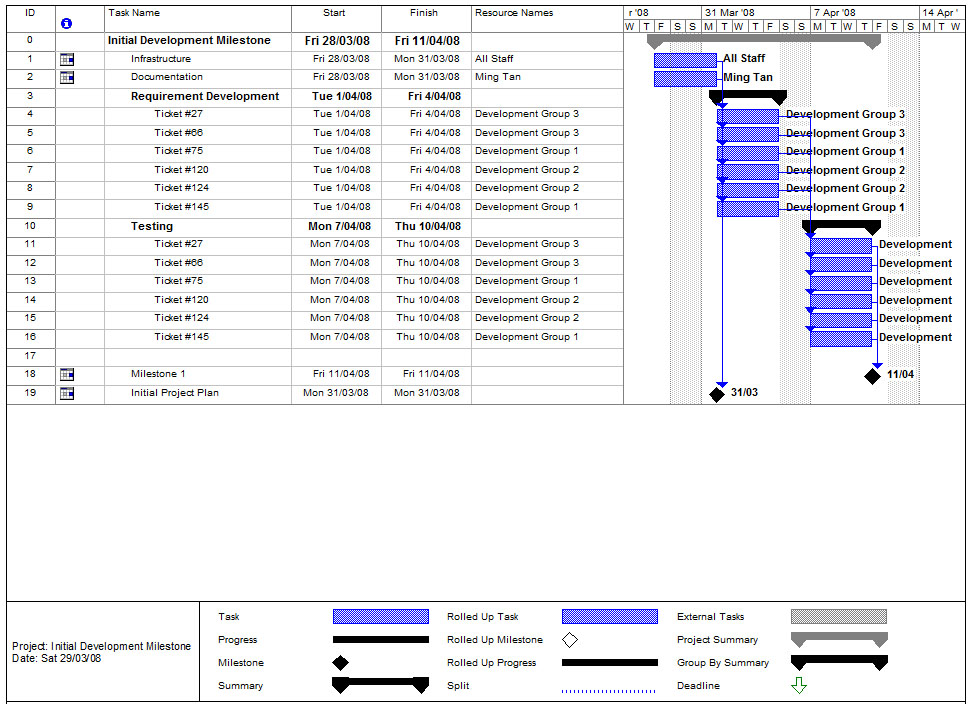
\includegraphics[angle=90,scale=0.5]{./schedule.jpg} 
\par\end{centering}
\caption{Gantt chart of project tasks for mileston 1}
\label{fig:schedule} 
\end{figure}

\newpage

\subsection{Milestone 2 - Work Activities}

\begin{itemize}
\item Ticket Investigation
\item Documentation
\item Ticket 138
\item Ticket 146
\item Ticket 42
\item Ticket 23
\item Database Design
\item Plugin System Design 
\item Testing
\end{itemize}

\subsubsection{Ticket Investigation}
	Each subgroup took various tickets, and investigated what would be needed to complete each ticket. This was done in order to discover which tasks would be best to undertake for this development iteration. Tickets 23, 40, 42, 138, 146 and 169 were investigated.\\
	
	Resource: All Development Staff
	Time Estimate: 5hrs

\subsubsection{Documentation}
	This involves the development and maintenance of existing documents for the project plan and any subsequent documents. During this iteration, the project plan was updated as well as documentation for testing processes and the git repository structure being added.\\
	
	Resource: Ming Tan, Alex Egan, Mohammad Bamogaddam
	Time Estimate: 8hrs

\subsubsection{Ticket 138}
	This ticket involves the testing of the existing improvements made to the radial and treemap views with filters to determine whether improvements are necessary.\\
	
	Resource: Development Group 1 (George Sainsbury, Alex Egan, Xiaodong Cui, Filimoni Lutunaika)
	Time Estimate: 4hrs

\subsubsection{Ticket 146}
	This ticket involves the addition of a script to allow for continuous testing of the code with test cases.\\
	
	Resource: Development Group 1 (George Sainsbury, Alex Egan, Xiaodong Cui, Filimoni Lutunaika )
	Time Estimate: 4hrs

\subsubsection{Ticket 42}
	This ticket involves the addition of job name, sequence name and shot name as metadata to allow for file searches via this information.\\
	
	Resource: Development Group 1 (George Sainsbury, Alex Egan, Xiaodong Cui, Filimoni Lutunaika )
	Time Estimate: 4hrs

\subsubsection{Ticket 23}
	This ticket involves the tagging or folksonomy of files and directories so that earth will be able to understand in a generic way the "RSP" file system concepts.\\

	Resource: Development Group 3 (Jonathan Velasco, Sahil Choujar, Ken S'ng Wong, Hemant Singh and Hill-Jian Huang)
	Time Estimate: 4hrs
	
\subsubsection{Database Design}
	This task involves reverse engineering of the existing database structure, and documenting it to allow for system changes to be made more easily.\\
	
	Resource: Development Group 3 (Jonathan Velasco, Sahil Choujar, Ken S'ng Wong, Hemant Singh and Hill-Jian Huang)
	Time Estimate: 4hrs

\subsubsection{Plugin System Design}
	This task involes the reverse engineering of the existing use of plugins in the system, and documenting how it is currently done and how it could best be structured.\\
	
	Resource: Development Group 2 (Ming Tan, Callum Ballie, Kun Zhou, Mohammad Bamogaddam and Yang Qing)
	Time Estimate: 4hrs
	
\subsubsection{Testing}
	Testing will be conducted on each of the tickets above, and testing scripts or unit tests will be created as necessary.\\
	
	Resource: All Development Groups
	Time Estimate: 8hrs

\subsubsection{Milestone 2 - Schedule Allocation}

The milestones and tasks are shown graphically in Figure \ref{fig:schedule2} below. This figure shows the relative times between the deadlines of the tasks required and also shows the estimated time for the completion of each individual tasks.\\

\begin{figure}[htp]
\begin{centering}
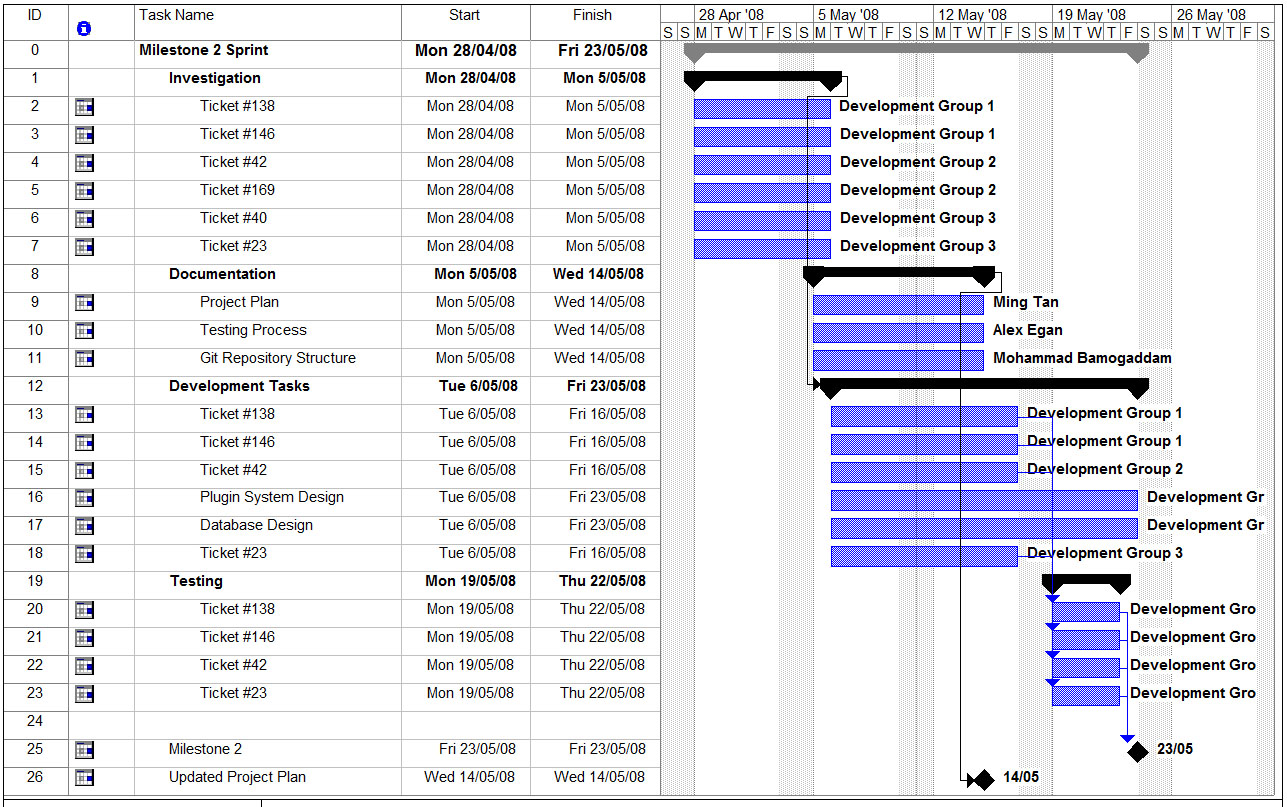
\includegraphics[angle=90,scale=0.5]{./schedule-milestone2.jpg} 
\par\end{centering}
\caption{Gantt chart of project tasks for milestone 2}
\label{fig:schedule2} 
\end{figure}

\subsection{Milestone 3 - Work Activities}

\begin{itemize}
\item Plugin Investigation
\item Plugin Processes
\item Ticket 27
\item Ticket 138
\item Ticket 42
\item Ticket 174 and Installation Package
\item Ticket 148
\item Daemon Remove Function
\item Ruby on Rails Tutorial
\item Planning Process and Templates
\item Requirement Process and Trac Process
\item Testing
\end{itemize}

\subsubsection{Plugin Investigation}
	The plugin system needs to be investigated with all the existing information about the plugins explained and to learn how to activate and update plugins.\\
	
	Resource: Development Group 3 (Jonathan Velasco, Sahil Choujar, Ken S'ng Wong, Hemant Singh and Hill-Jian Huang)
	Time Estimate: 5hrs

\subsubsection{Plugin Processes}
	This requires the use of the information acquired from the plugin investigation in order to learn how to edit the use and edit the existing plugins in addition to information on how to structure new plugins to be written.\\
	
	Resource: Development Group 3 (Jonathan Velasco, Sahil Choujar, Ken S'ng Wong, Hemant Singh and Hill-Jian Huang)
	Time Estimate: 8hrs

\subsubsection{Ticket 138}
	This ticket involves the testing of the existing improvements made to the radial and treemap views with filters to determine whether improvements are necessary.\\
	
	Resource: Development Group 1 (George Sainsbury, Alex Egan, Xiaodong Cui, Filimoni Lutunaika)
	Time Estimate: 4hrs

\subsubsection{Ticket 27}
	This ticket involves the addition of a script to allow for continuous testing of the code with test cases.\\
	
	Resource: Development Group 3 (Jonathan Velasco, Sahil Choujar, Ken S'ng Wong, Hemant Singh and Hill-Jian Huang)
	Time Estimate: 4hrs

\subsubsection{Ticket 42}
	This ticket involves the addition of job name, sequence name and shot name as metadata to allow for file searches via this information. This also further evolving the existing code to allow it be more generic and to be able to be used as a plugin.\\
	
	Resource: Development Group 2 (Ming Tan, Callum Ballie, Kun Zhou, Mohammad Bamogaddam and Yang Qing)
	Time Estimate: 4hrs

\subsubsection{Ticket 174 and Installation Package}
	This ticket involves the creation of an installation package and script to allow the installation of earth to be much simpler. It also looks at investigating gems for earth.\\

	Resource: Development Group 1 (George Sainsbury, Alex Egan, Xiaodong Cui, Filimoni Lutunaika)
	Time Estimate: 4hrs
	
\subsubsection{Daemon Remove Function}
	This ticket involes the implementation of the daemon remove function to allow directories to be removed from the daemon.\\

	Resource: Development Group 1 (George Sainsbury, Alex Egan, Xiaodong Cui, Filimoni Lutunaika)
	Time Estimate: 4hrs
	
\subsubsection{Ruby on Rails Tutorial}
	This task involes the addition of ruby on rails tutorial to bring the entire group up to speed with specific coding procedures that are helpful with the earth project.\\

	Resource: Development Group 2 (Ming Tan, Callum Ballie, Kun Zhou, Mohammad Bamogaddam and Yang Qing)
	Time Estimate: 4hrs

\subsubsection{Planning Process and Templates}
	This involes the creation of a process for planning at the start of each iteration as well as developing planning templates that each group can use.\\

	Resource: Development Group 2 (Ming Tan, Callum Ballie, Kun Zhou, Mohammad Bamogaddam and Yang Qing)
	Time Estimate: 4hrs
	
\subsubsection{Requirement Process and Trac Process}
	This task involves creating a process to create new requirements on the trac system and also how we can "close" off a ticket.\\
	
	Resource: Development Group 2 (Ming Tan, Callum Ballie, Kun Zhou, Mohammad Bamogaddam and Yang Qing)
	Time Estimate: 4hrs

\subsubsection{Testing}
	Testing will be conducted on each of the tickets above, and testing scripts or unit tests will be created as necessary.\\
	
	Resource: All Development Groups
	Time Estimate: 8hrs

\subsubsection{Milestone 3 - Schedule Allocation}

The milestones and tasks are shown graphically in Figure \ref{fig:schedule3} below. This figure shows the relative times between the deadlines of the tasks required and also shows the estimated time for the completion of each individual tasks.\\

\begin{figure}[htp]
\begin{centering}
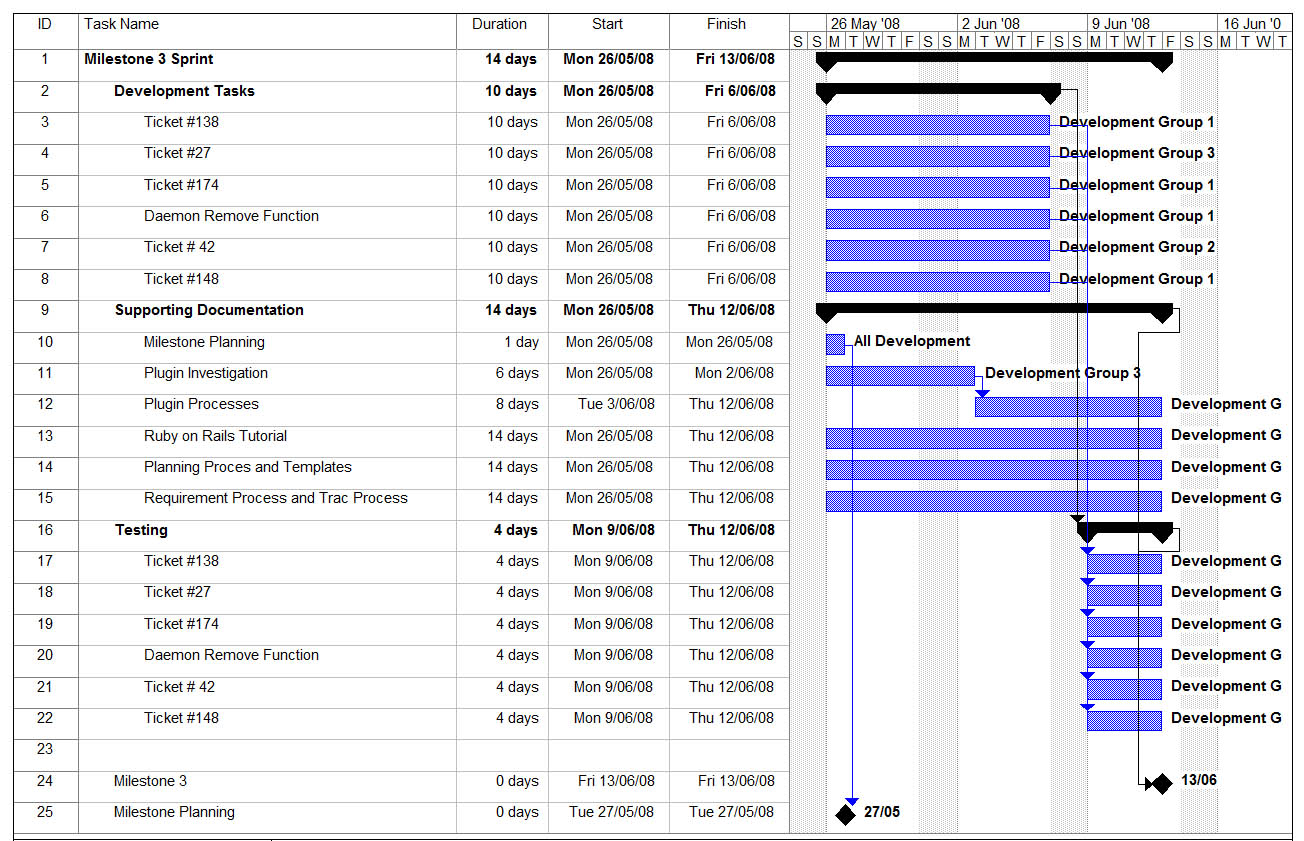
\includegraphics[angle=90,scale=0.5]{./schedule-milestone3.jpg} 
\par\end{centering}
\caption{Gantt chart of project tasks for milestone 3}
\label{fig:schedule3} 
\end{figure}

\subsection{Milestone 4 - Work Activities}

\begin{itemize}
\item Creation of API standards base for file monitor
\item Redevelopment of File Monitor with created API
\item Ticket 186
\item Ticket 75
\item Ticket 131
\item Ticket 174 and Installation Package
\item Ticket 176
\item Ticket 141
\item Ticket 90
\item Ticket 43
\item Ticket 154
\item Testing
\end{itemize}

\subsubsection{Creation of API standards base for file monitor}
	Create API standards base on the functionality of the file monitor (this includes DB but not GUI)\\
	
	Resource: Development Group 3 (Jonathan Velasco, Sahil Choujar, Ken S'ng Wong, Hemant Singh and Hill-Jian Huang)
	Time Estimate: 8hrs

\subsubsection{Redevelopment of File Monitor with created API}
	This is the recoding of File Monitor with the new API.\\
	
	Resource: Development Group 3 (Jonathan Velasco, Sahil Choujar, Ken S'ng Wong, Hemant Singh and Hill-Jian Huang)
	Time Estimate: 8hrs

\subsubsection{Ticket 131}
	This ticket aims to use real disk usage instead of byte size throughout the web application\\
	
	Resource: Development Group 1 (George Sainsbury, Alex Egan, Xiaodong Cui, Filimoni Lutunaika)
	Time Estimate: 4hrs
	
\subsubsection{Ticket 75}
	This ticket improves the sorting by name and size.\\
	
	Resource: Development Group 1 (George Sainsbury, Alex Egan, Xiaodong Cui, Filimoni Lutunaika)
	Time Estimate: 3hrs

\subsubsection{Ticket 174 and Installation Package}
	This ticket involves the creation of an installation package and script to allow the installation of earth to be much simpler. It also looks at investigating gems for earth.\\

	Resource: Development Group 1 (George Sainsbury, Alex Egan, Xiaodong Cui, Filimoni Lutunaika)
	Time Estimate: 3hrs
	
\subsubsection{Ticket 186}
	This ticket involes the implementation of the daemon remove function to allow directories to be removed from the daemon.\\

	Resource: Development Group 1 (George Sainsbury, Alex Egan, Xiaodong Cui, Filimoni Lutunaika)
	Time Estimate: 4hrs
	
\subsubsection{Ticket 176}
	This task requires plugin updating by combining all plugin installing functionality into one script "update_plugins".\\

	Resource: Development Group 2 (Ming Tan, Callum Ballie, Kun Zhou, Mohammad Bamogaddam and Yang Qing)
	Time Estimate: 8hrs

\subsubsection{Ticket 141}
	This involes adding a technical (architecture) overview of Earth to the wiki.\\

	Resource: Development Group 2 (Ming Tan, Callum Ballie, Kun Zhou, Mohammad Bamogaddam and Yang Qing)
	Time Estimate: 4hrs
	
\subsubsection{Ticket 90}
	This task involves creating a process to create new requirements on the trac system and also how we can "close" off a ticket.\\
	
	Resource: Development Group 2 (Ming Tan, Callum Ballie, Kun Zhou, Mohammad Bamogaddam and Yang Qing)
	Time Estimate: 1hr
	
\subsubsection{Ticket 43}
	This task involves creating an optional login feature for improved user tracking features.\\
	
	Resource: Development Group 2 (Ming Tan, Callum Ballie, Kun Zhou, Mohammad Bamogaddam and Yang Qing)
	Time Estimate: 4hrs
	
\subsubsection{Ticket 154}
	This task involves adding modified and user id to the directory level.\\
	
	Resource: Development Group 2 (Ming Tan, Callum Ballie, Kun Zhou, Mohammad Bamogaddam and Yang Qing)
	Time Estimate: 3hrs

\subsubsection{Testing}
	Testing will be conducted on each of the tickets above, and testing scripts or unit tests will be created as necessary.\\
	
	Resource: All Development Groups
	Time Estimate: 8hrs

\subsubsection{Milestone 4 - Schedule Allocation}

The milestones and tasks are shown graphically in Figure \ref{fig:schedule3} below. This figure shows the relative times between the deadlines of the tasks required and also shows the estimated time for the completion of each individual tasks.\\

\begin{figure}[htp]
\begin{centering}
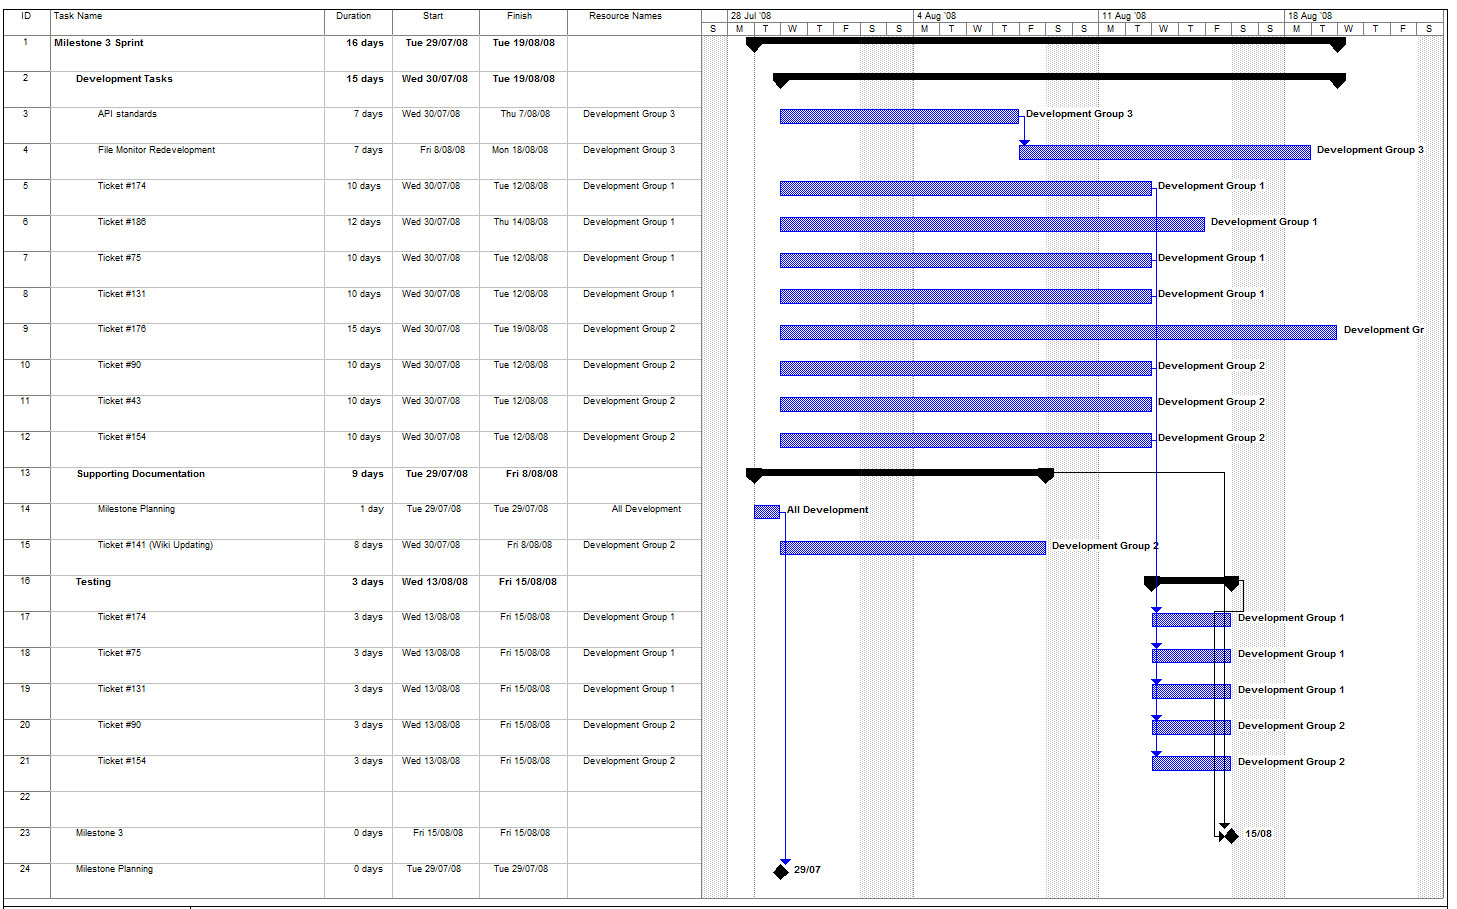
\includegraphics[angle=90,scale=0.5]{./schedule-milestone4.jpg} 
\par\end{centering}
\caption{Gantt chart of project tasks for milestone 3}
\label{fig:schedule3} 
\end{figure}

\newpage{}

\subsection{Milestone 5 - Work Activities}

\begin{itemize}
\item Further Development of API standards base for Plugins
\item Redevelopment of File Monitor with created API
\item Ticket 29
\item Ticket 75
\item Integration and Testing
\end{itemize}

\subsubsection{Further Development of API standards base for Plugins}
	Add on functionality to the API that was created for file monitor\\
	
	Resource: Development Group 5 (Xiaodong Cui, Filimoni Lutunaika, Ken S'ng Wong, Hill-Jian Huang, Kun Zhou, Mohammad Bamogaddam and Yang Qing)
	Time Estimate: 8hrs

\subsubsection{Redevelopment of File Monitor with created API}
	This is the recoding of File Monitor with the new API.\\
	
	Resource: Development Group 5 (Xiaodong Cui, Filimoni Lutunaika, Ken S'ng Wong, Hill-Jian Huang, Kun Zhou, Mohammad Bamogaddam and Yang Qing)
	Time Estimate: 8hrs
	
\subsubsection{Ticket 29}
	This task is to allow image data to be accessed more readily.
	
	Resource: Development Group 4 (Jonathan Velasco, Sahil Choujar, George Sainsbury, Alex Egan, Ming Tan, Callum Ballie)
	Time Estimate: 3hrs

\subsubsection{Ticket 75}
	This ticket improves the sorting by name and size.\\
	
	Resource: Development Group 4 (Jonathan Velasco, Sahil Choujar, George Sainsbury, Alex Egan, Ming Tan, Callum Ballie)
	Time Estimate: 3hrs

\subsubsection{Integration and Testing}
	Integration and testing will be conducted on each of the completed tickets from the existing milestones in order to ensure that once merged they are all still working.\\
	
	Resource: Development Group 4 (Jonathan Velasco, Sahil Choujar, George Sainsbury, Alex Egan, Ming Tan, Callum Ballie)
	Time Estimate: 8hrs

\subsubsection{Milestone 5 - Schedule Allocation}

The milestones and tasks are shown graphically in Figure \ref{fig:schedule5} below. This figure shows the relative times between the deadlines of the tasks required and also shows the estimated time for the completion of each individual tasks.\\

\begin{figure}[htp]
\begin{centering}
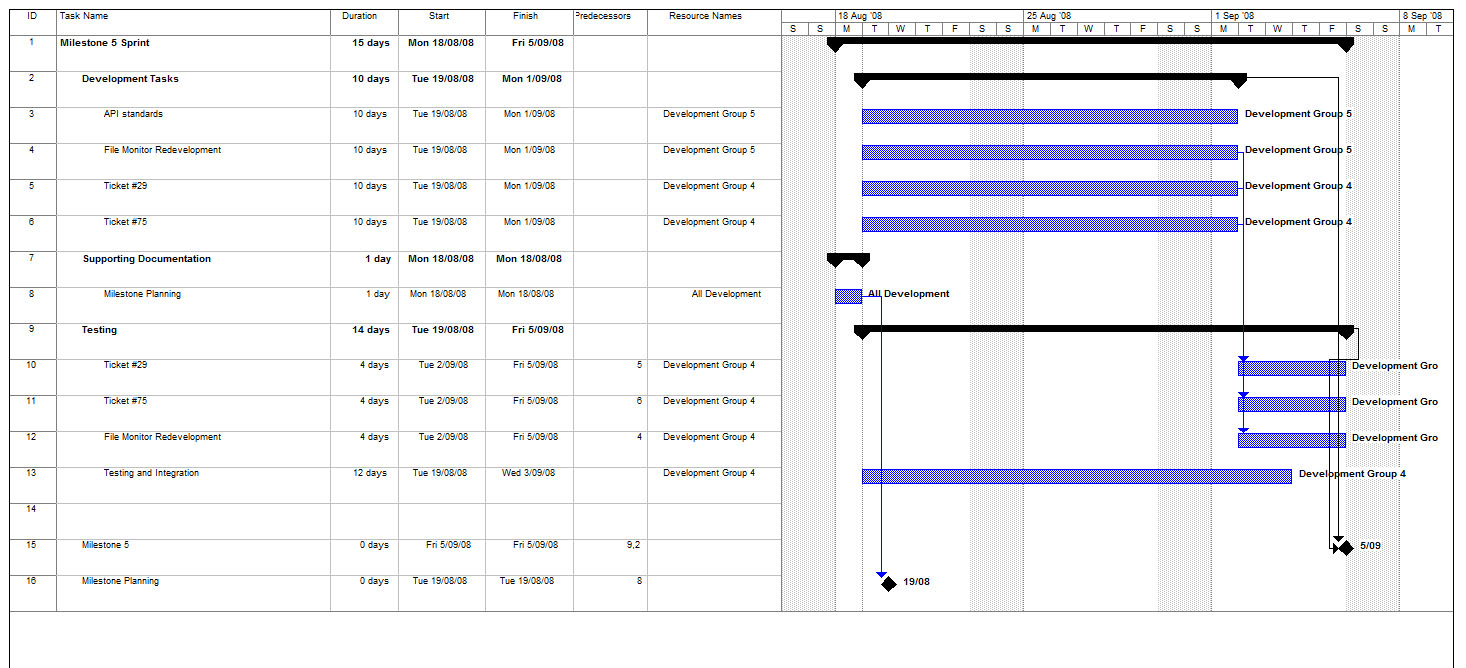
\includegraphics[angle=90,scale=0.5]{./schedule-milestone5.jpg} 
\par\end{centering}
\caption{Gantt chart of project tasks for milestone 5}
\label{fig:schedule5} 
\end{figure}

\newpage{}

\subsection{Milestone 6 - Work Activities}

\begin{itemize}
\item Further Development of Plugin System
\item Ticket 29
\item Ticket 75
\item Integration and Testing
\end{itemize}

\subsubsection{Further Development of Plugin System}
	Add on functionality to the API that was created for file monitor\\
	
	Resource: Development Group 5 (Xiaodong Cui, Filimoni Lutunaika, Ken S'ng Wong, Hill-Jian Huang, Kun Zhou, Mohammad Bamogaddam and Yang Qing)
	Time Estimate: 8hrs

\subsubsection{Ticket 29}
	This task is to allow image data to be accessed more readily. Addition to the GUI to display image data.
	
	Resource: Development Group 4 (Jonathan Velasco, Sahil Choujar, George Sainsbury, Alex Egan, Ming Tan, Callum Ballie)
	Time Estimate: 3hrs

\subsubsection{Ticket 75}
	Addition of pagenation to navigation view.\\
	
	Resource: Development Group 4 (Jonathan Velasco, Sahil Choujar, George Sainsbury, Alex Egan, Ming Tan, Callum Ballie)
	Time Estimate: 3hrs

\subsubsection{Integration and Testing}
	The current aim is to complete the above tasks toward the end of the second week of this development cycle and to integrate and test the functionality during the final week to lead into the testing during the final iteration.
	
	Resource: Development Group 4 (Jonathan Velasco, Sahil Choujar, George Sainsbury, Alex Egan, Ming Tan, Callum Ballie)
	Time Estimate: 8hrs

\subsubsection{Milestone 6 - Schedule Allocation}

The milestones and tasks are shown graphically in Figure \ref{fig:schedule5} below. This figure shows the relative times between the deadlines of the tasks required and also shows the estimated time for the completion of each individual tasks.\\

\begin{figure}[htp]
\begin{centering}
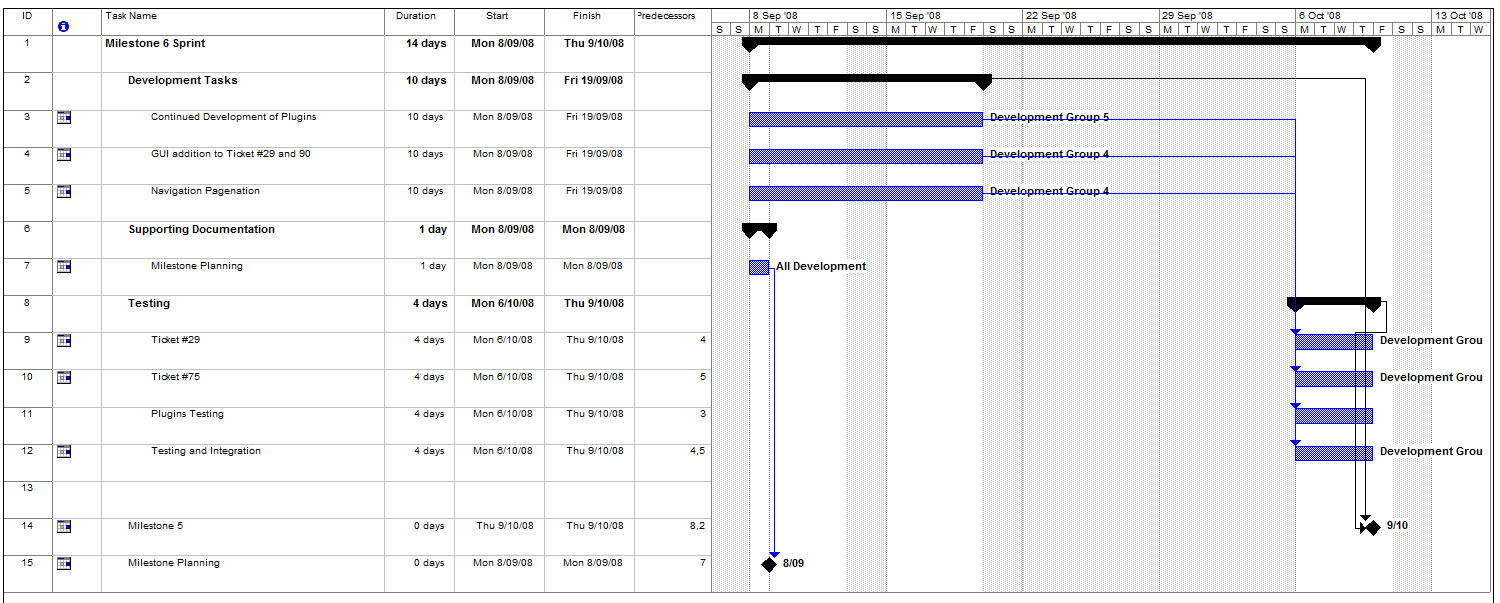
\includegraphics[angle=90,scale=0.5]{./schedule-milestone6.jpg} 
\par\end{centering}
\caption{Gantt chart of project tasks for milestone 6}
\label{fig:schedule5} 
\end{figure}

\newpage{}

\subsection{Milestones}

\subsubsection{Initial Features Update}

This milestone allows for the group members to familiarise themselves with the Earth code as well as the tools required to develop for Earth. In addition it allows a test run of the development sprint.\\
\textbf{Completion criteria:} The milestone has been achieved if tickets 27, 66, 75, 120, 127 and 145 are implemented and tested.
\\
\textbf{Due:} 11/04/08

\subsubsection{Development Sprint 2}

This milestone allows for more in depth tasks to be undertaken. \\
\textbf{Completion criteria:} The milestone has been achieved if tickets 23, 42, 138, and 146 are implemented and tested. In addition, there must be some design documentation for both the database and plugin systems.
\\
\textbf{Due:} 23/05/08

\subsubsection{Development Sprint 3}

This milestone allows for the completion of existing tickets from milestone 2 and the further development of supporting documentation. \\
\textbf{Completion criteria:} The milestone has been achieved if tickets 27, 42, 138, and 148 are implemented and tested. In addition, processes for ruby on rails, planning, requirements and plugins need to be completed.
\\
\textbf{Due:} 23/05/08

\subsubsection{Development Sprint 4}

This milestone allows for the further development of the plugin system with and improved API in addition to undertaking some GUI and database updates. \\
\textbf{Completion criteria:} The milestone has been achieved if tickets 75, 131, 174, 90, and 141 are completed. In addition tickets 176, 43, 154 and 186 should be near testing and/or undergoing testing. In addition, the creation of API standards base for file monitor and the redevelopment of file monitor should be undergoing testing.
\\
\textbf{Due:} 15/08/08

\subsubsection{Development Sprint 5}

This milestone allows for the further development of the plugin system with and improved API in addition to testing and integrating completed tickets. \\
\textbf{Completion criteria:} The milestone has been achieved if the plugin system has been implemented and allows for the installation of a plugin. In addition, the existing tickets should have been updated and tested.
\\
\textbf{Due:} 5/09/08

\subsubsection{Development Sprint 6}

This milestone allows for the further development of the plugin system with and improved API in addition to testing and integrating completed tickets. \\
\textbf{Completion criteria:} The milestone has been achieved if the plugin system has improved the installation of plugin systems. In addition, the existing tickets should have been updated and tested.
\\
\textbf{Due:} 10/10/08

\subsection{Resource Allocation}

As described in Section \ref{roles-and-responsibilities}, people will be allocated to each task in the following fashion:

\begin{itemize}
	
\item \textbf{Development Group 1:} George Sainsbury, Alex Egan, Xiaodong Cui, Filimoni Lutunaika \\

\item \textbf{Development Group 2:} Ming Tan, Callum Ballie, Kun Zhou, Mohammad Bamogaddam and Yang Qing\\

\item \textbf{Development Group 3:} Jonathan Velasco, Sahil Choujar, Ken S'ng Wong, Hemant Singh and Hill-Jian Huang\\

\item \textbf{Development Group 4:} Jonathan Velasco, Sahil Choujar, George Sainsbury, Alex Egan, Ming Tan, Callum Ballie\\

\item \textbf{Development Group 5:} Xiaodong Cui, Filimoni Lutunaika, Ken S'ng Wong, Hill-Jian Huang, Kun Zhou, Mohammad Bamogaddam and Yang Qing\\

\item \textbf{Documentation:} Ming Tan, Alex Egan, Mohammad Bamogaddam\\

\end{itemize}

If a task is completed early, or it is noted that less people are required to complete a task on schedule, they will be reallocated to other tasks.\\

\section{Supporting Plans}

\subsection{Git Repository Process}

\subsubsection{Human Resources Allocation:}
\begin{itemize}	
\item Each group will have a GitHub leader who is responsible for their group's copy of the central repository.
\item The GitHub leaders will be responsible for the central repository.
\end{itemize}

\subsubsection{Creation:}
\begin{itemize}	
\item At first, the GitHub manager should fork the origin from RSP repository. So, we will have: manager/earth
\item Then, GitHub leaders should fork (clone) their masters from the origin (i.e. manager/earth). So, we will have: leader1/earth, leader2/earth and leader3/earth
\item each leader should give all his group members permitions to push their group fork
\item Then, each group member should only clone the group's master fork to his local PC (i.e. leader1/earth, leader2/earth and leader3/earth).
\end{itemize}

\subsubsection{Upon Completion of a task:}
\begin{itemize}	
\item He pulls the latest changes from the group's master. (git pull)
\item Test his task locally.
\item Pushes the changes.
\item Sends a pull request to the group GitHub leader (and all other group memebers). This request should include (at least): related task number or description, files changed, related ticket numbers. (this really a notification not a request since he already pushes his changes)
\end{itemize}

\subsubsection{Upon pull request to Github Leader:}
\begin{itemize}	
\item The group GitHub leader reviews the changes in terms of: documentation standards, etc.
\item Performs the automated test to make sure that nothing is corrupted. (he could fully test the changes and approve it "for discussion in the meeting")
\item If the changes are approved: Sends a pull request to: all group members & GitHub manager about the changes:  related task number or description, files changed, related ticket numbers and person responsible.
\item If the changes are not approved: Reverts back the group's master  to its status before these changes are committed, and sends an email to the group member clarifying the reasons of rejecting the changes.
\end{itemize}

\subsubsection{When the GitHub manager receives a pull request from a GitHub leader:}
\begin{itemize}	
\item The Github manager pulls the latest changes from that group's master. (this could includes any necessary merges)
\item The GitHub manager performs an automated final test. (should be specified) 
\item If it passed the test successfully, sends a pull request to all other GitHub leaders so that they pull the latest changes to their forks.
(He could marks a version??)
\item If it does not pass the test: Reverts back the origin to its state before these changes, and inform the group GitHub leader by an email about the reasons. (or from the beginning, make a fake fork or branch for testing)
\end{itemize}

\subsubsection{Milestone Completion:}
\begin{itemize}	
\item The GitHub manager marks a version/release 
\item He sends a pull request to Earth people. This should contain: Milestone features, (for discussion)
\end{itemize}

\end{document}
